\documentclass[a4paper,12pt]{article} % Document class

% Packages
\usepackage[utf8]{inputenc} % Encoding
\usepackage{amsmath} % For mathematical formulas
\usepackage{graphicx} % For including images
\usepackage{hyperref} % For hyperlinks
\usepackage{titling} % For custom title
\usepackage{pdflscape} % For landscape pages
\usepackage{tabularx} % For flexible column widths
\usepackage[margin=2.5cm]{geometry} % Adjust the margin here (e.g., 2.5cm)
\usepackage{graphicx} % For including images
\usepackage{multirow}
\usepackage{listings} % import and format code from an external file


% Set default path for images
\graphicspath{{../img/}}

% Prevent hyphenation globally
\hyphenpenalty=10000
\exhyphenpenalty=10000

% LaTeX HTML content import
\lstset{
    language=HTML,
    inputencoding=utf8, % Ensure the input encoding is set correctly
    basicstyle=\ttfamily\small,
    breaklines=true,
    columns=fullflexible,
    literate={<}{{\textless}}1 
             {>}{{\textgreater}}1
             {é}{{\'e}}1  % Map é to its LaTeX command
             {&}{{\&}}1   % Ensure & is properly escaped
             {€}{{\texteuro}}1  % Map € to its LaTeX command
}


\title{Web Technologies \\
        \large{Exercise Sheet 1 -- Web-Shop - Presentations and HTML}} % Title
\author{Team 3: Jiahui~Dai, Yana~Halamakh, Wei~Wei~Tang} % Author
\date{\today} % Date

\begin{document}

\maketitle % Create title
\hrule % Create a horizontal line
\tableofcontents % Create table of contents
\textbf{For a detailed implementation, refer to the source code.}
\newpage


\section{General Questions}
\subsection{Task 1.1}


\subsection{Task 1.2}
\subsection{Communication Layers}

\begin{center}
    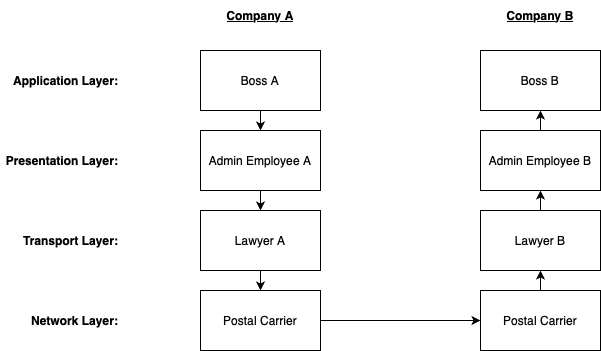
\includegraphics[width=.8\textwidth]{communication-layers.drawio.png}
\end{center}

% Application Layer: The bosses send messages through their administrative employees (Admin A and Admin B).
% Presentation Layer: Responsible for ensuring the message is encrypted before sending and decrypted upon receiving.
% Transport Layer: Handles the transmission of messages between Admin A and Admin B.
% Network Layer: Responsible for the routing and addressing of messages over the internet.

\section{Conceptual Model}
Please refer to  Figure~\ref{fig:task2} for the structural workflow model of our website.
% To redraw diagram.

\begin{figure}[h]
    \centering
    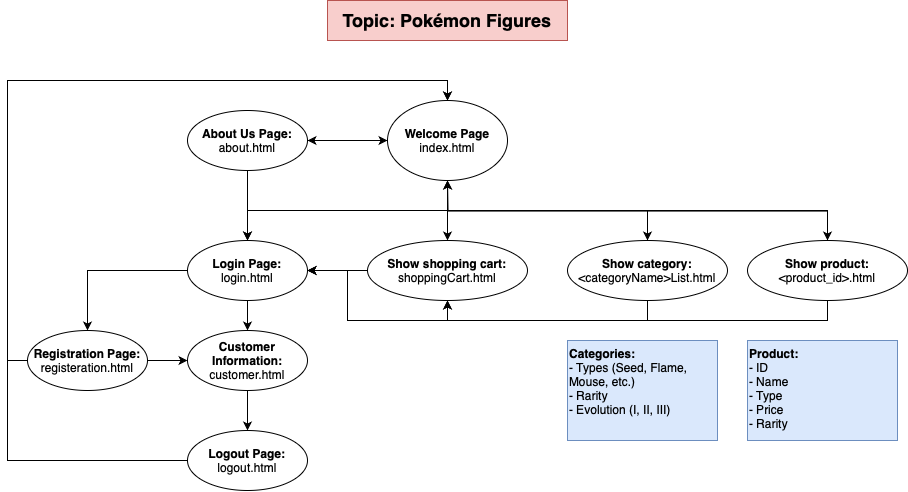
\includegraphics[width=\textwidth]{conceptual-model.drawio.png} % Adjust the path and file name
    \caption{Conceptual Model for Web-Shop}
    \label{fig:task2}
\end{figure}

\section{\texttt{index.html}}

\lstinputlisting[language=HTML]{../../src/index.html}
\section{Freestyle}

\begin{itemize}
    \item Products and orders are searchable by their IDs.
    \item Products can be filtered by type.
    \item Users can add and update billing and shipping addresses.
    \item Admins can validate or invalidate coupon codes (bug in display changes for coupons).
    \item Guest shopping carts are transferred to registered accounts.
\end{itemize}

\section{Final Steps}

\paragraph{Bugs fixed}
\begin{enumerate}
    \item Added a hamburger menu for mobile users (fix for Exercise-Sheet-3 Style Modification).
    \item Fixed product additions to the collection list (fix for Exercise-Sheet-3 Collection List).
    \item Corrected product display and \texttt{pid} query handling in \texttt{product.php} (fix for Exercise-Sheet-4 Category and Product Page).
    \item Fixed the randomized product page redirection (feature from Exercise-Sheet-3) to work with the updated \texttt{product.php} and its product ID query.
\end{enumerate}

\paragraph{Updates}
\begin{itemize}
    \item Standardized CSS classes.
    \item Deprecated collection list in favor of the shopping cart feature.
    \item Added a main product page displaying all products with search and filter options, and added functionality to add products to the cart.
\end{itemize}
\section{\texttt{logout.html}}

\lstinputlisting[language=HTML]{../../src/logout.html}
\section{\texttt{customer.html}}

\lstinputlisting[language=HTML]{../../src/customer.html}
\section{\texttt{about.html}}

\lstinputlisting[language=HTML]{../../src/about.html}
\section{\texttt{<categoryName>List.html}}

\begin{tabular}{|c|c|}
    \hline
    \textbf{Main Categories} & \textbf{Sub-Categories}\\
    \hline
    % Type
    \multirow{3}{*}{Type} & Grass \\
    \cline{2-2}
    & Poison \\
    \cline{2-2}
    & Water \\
    \hline
    % Category
    \multirow{4}{*}{Category} & Seed \\
    \cline{2-2}
    & Tiny Turtle \\
    \cline{2-2}
    & Turtle \\
    \cline{2-2}
    & Shellfish \\
    \hline
\end{tabular}

% Code imports
\subsection{\texttt{mainList.html}}
\lstinputlisting[language=HTML]{../../src/categoryList/mainList.html}

% 1. Category
\newpage
\subsection{Category 1: \texttt{categoryList.html}}
\lstinputlisting[language=HTML]{../../src/categoryList/categories/categoryList.html}

\newpage
\subsubsection{Sub-Category 1: \texttt{seed.html}}
\lstinputlisting[language=HTML]{../../src/categoryList/categories/seed.html}
\newpage
\subsubsection{Sub-Category 2: \texttt{shellfish.html}}
\lstinputlisting[language=HTML]{../../src/categoryList/categories/shellfish.html}
\newpage
\subsubsection{Sub-Category 3: \texttt{tiny-turtle.html}}
\lstinputlisting[language=HTML]{../../src/categoryList/categories/tiny-turtle.html}
\newpage
\subsubsection{Sub-Category 4: \texttt{turtle.html}}
\lstinputlisting[language=HTML]{../../src/categoryList/categories/turtle.html}


% 2. Types
\newpage
\subsection{Category 2: \texttt{typeList.html}}
\lstinputlisting[language=HTML]{../../src/categoryList/types/typeList.html}

\newpage
\subsubsection{Sub-Category 1: \texttt{grass.html}}
\lstinputlisting[language=HTML]{../../src/categoryList/types/grass.html}
\newpage
\subsubsection{Sub-Category 2: \texttt{poison.html}}
\lstinputlisting[language=HTML]{../../src/categoryList/types/poison.html}
\newpage
\subsubsection{Sub-Category 3: \texttt{water.html}}
\lstinputlisting[language=HTML]{../../src/categoryList/types/water.html}
\section{\texttt{<product\_id>.html}} 
\begin{tabular}{|c|c|}
    \hline
    \textbf{ID} & \textbf{Name}\\
    \hline
    \#0001 & Bulbasaur\\
    \hline
    \#0002 & Ivysaur\\
    \hline
    \#0003 & Venusaur\\
    \hline
    \#0007 & Squirtle\\
    \hline
    \#0008 & Wartortle\\
    \hline
    \#0009 & Blastoise\\
    \hline
\end{tabular}

\subsection{\texttt{0001.html}}
\lstinputlisting[language=HTML]{../../src/product_id/0001.html}
\newpage
\subsection{\texttt{0002.html}}
\lstinputlisting[language=HTML]{../../src/product_id/0002.html}
\newpage
\subsection{\texttt{0003.html}}
\lstinputlisting[language=HTML]{../../src/product_id/0003.html}
\newpage
\subsection{\texttt{0007.html}}
\lstinputlisting[language=HTML]{../../src/product_id/0007.html}
\newpage
\subsection{\texttt{0008.html}}
\lstinputlisting[language=HTML]{../../src/product_id/0008.html}
\newpage
\subsection{\texttt{0009.html}}
\lstinputlisting[language=HTML]{../../src/product_id/0009.html}



% END OF DOCUMENT
\begin{center}
    \vspace{5em}
    \textbf{END OF DOCUMENT}
\end{center}


\end{document}
